\documentclass[letterpaper,11pt]{article}
\usepackage[utf8]{inputenc}
\usepackage[T1]{fontenc}
\IfFileExists{spanish.ldf}{%
  \usepackage[spanish,es-tabla,es-nodecimaldot]{babel}
}{%
  \usepackage{babel}
  \babelprovide[import,main]{spanish}
}
\usepackage{lmodern,microtype}
\usepackage[margin=2.5cm]{geometry}
\usepackage{amsmath,amssymb,booktabs,tabularx,array,enumitem,xcolor,graphicx}
\usepackage{tikz}
\usetikzlibrary{babel,positioning,arrows.meta,shapes.geometric}
\usepackage[numbers,sort&compress]{natbib}
\usepackage[hidelinks]{hyperref}
\setlength{\parskip}{0.45em}\setlength{\parindent}{0pt}
\setlist{nosep,topsep=0.3em}
\renewcommand{\arraystretch}{1.15}
\newcolumntype{Y}{>{\raggedright\arraybackslash}X}
\newcommand{\passuno}{\texttt{pass@1}}
\newcommand{\passk}{\texttt{pass@}\ensuremath{k}}
% Decisiones aún abiertas del grupo (ver TODO de reunión).
\newcommand{\pd}[1]{\textcolor{orange!70!black}{\textit{[Por decidir: #1]}}}

\title{\textbf{Entrenar un LLM pequeño para resolver Sudoku: comparación de SFT, DPO y RLVR sobre un entorno verificable}\\[0.3em]
\large Propuesta inicial -- Entrega 1}
\author{Lilly Guevara \and Cristian Hinostroza \and Juan Moya \and Dan Villablanca}
\date{IIC-3694 Inteligencia Artificial Generativa -- 11 de noviembre de 2026}

\begin{document}
\maketitle

\begin{abstract}
Proponemos comparar cuatro estrategias de post-entrenamiento para el modelo \texttt{Qwen3.5-2B} —SFT, SFT seguido de aprendizaje por refuerzo con recompensas verificables (SFT$\to$RLVR mediante GRPO), RLVR puro y DPO— junto con el modelo base como línea de control, evaluando todos los enfoques sobre un mismo entorno de Sudoku verificable y bajo un presupuesto de cómputo equivalente. Como contribución principal, diseñamos un currículo de dificultad progresiva basado en el número de celdas vacías para el entrenamiento con RLVR, contrastando su desempeño frente al muestreo uniforme de dificultades mezcladas. Apoyándonos en el entorno, los conjuntos de datos y la línea base preliminar del Desafío, buscamos responder cinco preguntas clave: (i) si una etapa previa de SFT acelera o restringe la exploración durante RLVR; (ii) en qué medida generaliza cada estrategia hacia la partición de prueba y hacia niveles de dificultad no vistos; (iii) si el currículo por celdas vacías mejora la eficiencia muestral y el rendimiento final; (iv) si las capacidades de razonamiento adquiridas se transfieren a entornos desarrollados por otros grupos del curso; y (v) si emergen comportamientos de explotación del verificador (\emph{reward hacking}). Finalmente, documentaremos el ciclo completo de refinamiento iterativo —entrenar, inspeccionar trazas, parchar el verificador y reentrenar— acompañado de una auditoría manual sobre las trazas exitosas.
\end{abstract}

\section{Introducción y motivación}
El aprendizaje reforzado con recompensas verificables (RLVR) ha pasado a ser una pieza central del post-entrenamiento de modelos de razonamiento \citep{lambert2024tulu3,deepseekr1}. Su ingrediente clave es un verificador automático que sirve como recompensa. Esto lo hace atractivo, pero también frágil: un verificador imperfecto puede ser explotado por la política \citep{skalse2022reward}. Además, hay evidencia mixta sobre si RLVR agrega capacidades o solo afina las que el modelo ya posee \citep{yue2025limit}, y sobre el rol del SFT previo: \citet{chu2025sft} observan que el SFT tiende a memorizar mientras que RL generaliza mejor a variantes no vistas, aunque el SFT estabiliza el formato de salida y facilita el RL posterior, como en el arranque en frío de DeepSeek-R1 \citep{deepseekr1}.

Estas preguntas son difíciles de estudiar a escala de laboratorio de frontera, pero se pueden abordar con un modelo pequeño y un entorno barato de verificar. En el Desafío construimos un harness de Sudoku ($4\times4$, $6\times6$ y $9\times9$, tres niveles de dificultad) cuya respuesta se verifica por construcción. El Sudoku es un problema de razonamiento con restricciones, de varios pasos, que Qwen3.5-2B resuelve mal: en nuestra línea base obtiene un \passuno\ de 6,9\,\% y ningún acierto en $9\times9$. Este proyecto usa ese entorno para comparar estrategias de entrenamiento de forma controlada. Entrenaremos solo con $4\times4$ y $6\times6$; los $9\times9$ quedan fuera del entrenamiento y se usan únicamente para evaluar.

\textbf{Objetivo y contribuciones.} Buscamos comparar de forma controlada, sobre este entorno, las cuatro estrategias de entrenamiento (SFT, SFT$\to$RLVR, RLVR y DPO) y el modelo base como control, es decir, los cinco caminos que define el enunciado \citep{enunciadoproyecto2026}. Las contribuciones esperadas son: (i) una comparación de SFT, DPO y RLVR a cómputo comparable, con \passuno\ y \passk\ por nivel de dificultad; (ii) un currículo por número de celdas vacías para GRPO, evaluado contra la mezcla uniforme de dificultades, y (iii) un registro del ciclo de iteración y una auditoría manual de trazas exitosas para detectar \emph{reward hacking}.

\section{Revisión bibliográfica}
\textbf{Entornos verificables.} Reasoning Gym \citep{stojanovski2025reasoninggym} ofrece generadores de tareas con verificadores y dificultad configurable; nuestro generador de Sudoku adapta el suyo. AgentGym \citep{xi2025agentgym} sigue la misma filosofía para agentes con herramientas.

\textbf{Algoritmos.} PPO \citep{schulman2017ppo} es la base del RLHF de InstructGPT \citep{ouyang2022instructgpt}. GRPO \citep{shao2024deepseekmath} elimina el crítico y estima la ventaja comparando las recompensas de un grupo de respuestas a un mismo prompt; así se usó en DeepSeek-R1 \citep{deepseekr1}. Trabajos posteriores analizan sesgos de GRPO, como la normalización por longitud y por desviación estándar \citep{liu2025drgrpo}, y proponen mejoras prácticas, como filtrar grupos sin señal y recortar de forma asimétrica \citep{yu2025dapo}. DPO \citep{rafailov2023dpo} optimiza directamente sobre pares de preferencia, sin modelo de recompensa ni muestreo en línea, y es de bajo costo. Para SFT y DPO con pocos recursos usaremos LoRA \citep{hu2022lora} sobre las implementaciones de TRL \citep{vonwerra2020trl}.

\textbf{Currículo.} El aprendizaje por currículo presenta ejemplos de menor a mayor dificultad \citep{bengio2009curriculum}. En RLVR para LLM, Kimi k1.5 usa muestreo por currículo y priorizado \citep{kimi2025k15}, y DAPO filtra grupos donde todas las respuestas reciben la misma recompensa \citep{yu2025dapo}. Nuestro entorno permite controlar la dificultad con una variable explícita y barata, el número de celdas vacías, lo que facilita estudiar el currículo de forma controlada.

\textbf{SFT frente a RL.} \citet{chu2025sft} comparan ambos post-entrenamientos en un juego de cartas aritmético y en una tarea de navegación: RL generaliza a variantes no vistas de las reglas, mientras que SFT tiende a memorizar; aun así, el SFT previo estabiliza el formato de salida y permite que RL obtenga sus ganancias. Nuestros caminos 2 a 4 ponen a prueba esta observación en otro dominio y con un modelo de lenguaje pequeño.

\textbf{Sudoku y LLM.} Sudoku-Bench \citep{seely2025sudokubench} reúne 100 variantes de Sudoku y reporta que los LLM de frontera resuelven menos del 15\,\% sin ayuda. A diferencia de ese trabajo, que solo evalúa, usamos Sudokus clásicos de tamaño y dificultad controlados como entorno de entrenamiento.

\textbf{Qué aporta RLVR.} \citet{yue2025limit} reportan que, medido con \passk\ para $k$ grande \citep{chen2021codex}, los modelos entrenados con RLVR no superan al modelo base. Esto motiva reportar \passk\ además de \passuno, y estudiar en qué zona de dificultad hay señal.

\textbf{Reward hacking y auditoría.} \citet{skalse2022reward} formalizan el \emph{reward hacking}. En código, SWE-Bench+ \citep{aleithan2024swebenchplus} mostró que una parte importante de los aciertos aparentes no era genuina, lo que motiva la auditoría manual de trazas exitosas que pide el enunciado \citep{enunciadoproyecto2026}.

\textbf{Nuestra posición.} A diferencia de estos trabajos, combinamos en un mismo entorno barato de verificar la comparación de las cuatro estrategias de entrenamiento frente al modelo base, un currículo con una variable de dificultad explícita y una auditoría de los aciertos.

\section{Entorno a utilizar}
Emplearemos el \emph{harness} desarrollado por nuestro grupo para el Desafío (cuyo repositorio será publicado próximamente) para entrenar el modelo \texttt{Qwen/Qwen3.5-2B}.

\begin{itemize}
  \item \textbf{Interfaz:} \texttt{reward(prompt, completion) -> float}. El modelo puede razonar libremente antes de responder, pero su salida debe finalizar con un único bloque \texttt{<answer>...</answer>} que contenga el tablero como una matriz JSON de $N\times N$ enteros. El \emph{parser} invalida la respuesta ($\text{format}=0$) si existe texto posterior a dicho bloque, si aparece más de una etiqueta \texttt{<answer>} o si esta se encuentra anidada dentro del bloque de razonamiento (\texttt{<think>}). De este modo, se evita que el modelo burle al verificador entregando múltiples soluciones candidatas.

  \item \textbf{Tareas:} \emph{Splits} de \emph{train/eval/test} disjuntas entre sí, compuestas por tableros con solución única distribuidos en tres tamaños y tres niveles de dificultad por tamaño.

  \item \textbf{Función de recompensa:} Se define como 
  \[
    \text{reward} = \text{format} \cdot (w_{\text{fill}} \cdot \text{fill} \cdot \text{clues\_frac} + w_{\text{solve}} \cdot \text{solved}),
  \]
  sujeta a $w_{\text{fill}} + w_{\text{solve}} = 1$ (por defecto, $0.5$ cada uno). Dado que todos los factores pertenecen al intervalo $[0,1]$, la recompensa resultante también está acotada en dicho rango. Cada componente evalúa un aspecto específico:
  \begin{itemize}
    \item $\text{format} \in \{0,1\}$: Toma el valor $1$ si la salida respeta estrictamente el contrato estructural descrito; en caso contrario, anula la recompensa total.
    \item $\text{clues\_frac} \in [0,1]$: Proporción de pistas iniciales del tablero que se mantienen intactas, penalizando errores al copiar la entrada.
    \item $\text{fill} \in [0,1]$: Proporción de celdas originalmente vacías que coinciden con la solución única. Actúa como crédito parcial por avance, contabilizando como error tanto los ceros como los valores fuera de rango.
    \item $\text{solved} \in \{0,1\}$: Toma el valor $1$ si el tablero cumple las reglas del Sudoku (filas, columnas y subcuadrículas válidas) y conserva todas las pistas originales, aceptando cualquier solución válida.
  \end{itemize}
  Así, una solución completa otorga $\text{reward}=1$, mientras que un tablero bien formateado que conserva las pistas pero acierta solo $40$ de $50$ celdas vacías obtiene $0.5 \cdot 0.8 = 0.4$. Como línea de comparación (\emph{ablation}), evaluaremos también una variante binaria ($\text{reward} = \text{format} \cdot \text{solved}$) para aislar el impacto del crédito parcial.

  \item \textbf{Datos generados:} Trazas de razonamiento correctas para SFT y pares de respuestas correcta/incorrecta para DPO, generados sobre el \emph{split} de entrenamiento utilizando \texttt{Qwen3.5-9B} como modelo profesor y filtrados mediante el verificador.
\end{itemize}

\textbf{\emph{Baseline} preliminar.} Para cada tarea se muestrean $n$ respuestas independientes del modelo (con temperatura $T > 0$) y se evalúan con el verificador; a partir de la proporción de aciertos se calcula el estimador insesgado de \passk\ (con $k \le n$) siguiendo a \citet{chen2021codex}. En una evaluación inicial del modelo de 9B para el Desafío ($n=8$ muestras en $10$ tareas de validación por combinación de tamaño y dificultad, totalizando $80$ respuestas por celda), solo $12$ de las $90$ tareas presentaron resultados mixtos (combinación de aciertos y fallos). Estas se concentraron exclusivamente en los tableros de $4\times4$ (en todos sus niveles) y en los de $6\times6$ de dificultad \emph{easy} y \emph{medium}. Por el contrario, el modelo no resolvió ninguna instancia en $6\times6$ \emph{hard} ni en los tableros de $9\times9$. Esta ausencia de señal de aprendizaje, sumada al alto costo computacional de generar datos y entrenar sobre tableros de $9\times9$, justifica descartar dicho tamaño en la etapa de entrenamiento. Actualmente estamos recalculando estas métricas con un conjunto de datos ampliado, por lo que los valores reportados son provisionales y serán actualizados en la Entrega~2.

\section{Propuesta de investigación}\label{sec:diseno}
\subsection{Preguntas e hipótesis}
\begin{description}[leftmargin=0pt]
  \item[P1.] ¿El SFT previo acelera o limita el aprendizaje con RLVR? \emph{H1:} SFT$\to$RLVR converge más rápido que solo RLVR en la zona aprendible, pero con \passk\ final similar o menor para $k$ grande.
  \item[P2.] ¿Cuánto generaliza cada estrategia a la partición de prueba, a niveles no vistos y a un tamaño de tablero no visto ($9\times9$)? \emph{H2:} RLVR generaliza mejor que SFT y DPO a niveles no vistos; SFT tiende a memorizar el formato de las trazas del profesor.
  \item[P3.] ¿Aparece \emph{reward hacking} y bajo qué condiciones? \emph{H3:} aparecerá más con recompensa parcial que con la binaria, por ejemplo respuestas que copian pistas y adivinan el resto, o que explotan el formato.
  \item[P4.] ¿Un currículo por número de celdas vacías mejora el entrenamiento con RLVR frente a mezclar dificultades? \emph{H4:} un currículo adaptativo alcanza la misma recompensa con menos pasos y llega a niveles que el entrenamiento con mezcla uniforme no resuelve (por ejemplo $6\times6$ \emph{hard}), porque mantiene los grupos de GRPO en la zona con señal.
  \item[P5.] ¿Lo aprendido en Sudoku se transfiere, o se pierde, en tareas de razonamiento de otros entornos? \emph{H5:} el SFT degrada más el desempeño fuera de dominio que RLVR, que se mantiene más cerca del modelo base.
\end{description}

\subsection{Experimento central}
Los cinco caminos (el modelo base como control y cuatro estrategias de entrenamiento) se evalúan sobre el mismo entorno, con presupuesto de cómputo comparable (criterio en la sección~\ref{sec:computo}).
\begin{center}\small
\begin{tabularx}{\linewidth}{@{}clY@{}}
\toprule
\# & Camino & Descripción \\
\midrule
1 & Base (control) & Qwen3.5-2B sin entrenamiento adicional. \\
2 & SFT & SFT con LoRA sobre trazas correctas del profesor. \\
3 & SFT$\to$RLVR & Camino 2 seguido de GRPO con el verificador como recompensa. \\
4 & RLVR & GRPO directamente desde el modelo base. \\
5 & DPO & DPO con LoRA sobre pares correcta/incorrecta. \\
\bottomrule
\end{tabularx}
\end{center}

\subsection{Diseño y ablations}
\begin{itemize}
  \item \textbf{Datos de entrenamiento y evaluación.} Se entrena solo con $4\times4$ y $6\times6$ (todos los niveles, ya que el currículo busca llegar a $6\times6$ \emph{hard}); los caminos 2 a 5 usan una mezcla fija de dificultades. Los $9\times9$ se excluyen del entrenamiento. Por la línea base, la zona con señal es $4\times4$ y $6\times6$ \emph{easy}/\emph{medium}.
  \item \textbf{Evaluación en $9\times9$.} Se mantiene en la evaluación para medir generalización a un tamaño no visto en el entrenamiento. Como con la línea base actual se espera \passuno\ cercano a cero, en este tamaño se reporta también la fracción de celdas vacías completadas correctamente, que puede mostrar avances parciales aunque ningún tablero se resuelva completo.
  \item \textbf{Ablations (RLVR).} Por el costo de GRPO se estudian solo dos ablations, la forma de la recompensa (binaria vs.\ parcial), que pone a prueba H3, y el tamaño de grupo $G$ (8 vs.\ 16), que cambia la probabilidad de que un grupo tenga respuestas correctas e incorrectas y, por lo tanto, señal. El coeficiente KL se fija en un único valor, y la mezcla de dificultades ya se compara en la contribución.
  \item \textbf{Contribución (nivel 3): currículo por celdas vacías.} En lugar de los tres niveles gruesos, se usa el número de celdas vacías como eje continuo de dificultad. Se entrena GRPO con tres variantes de muestreo de tareas: (a) \emph{mezcla uniforme} sobre todo el rango (baseline); (b) \emph{currículo fijo}, con un calendario creciente de celdas vacías; (c) \emph{currículo adaptativo}, que avanza al siguiente rango cuando el \passuno\ de entrenamiento reciente supera un umbral $\tau$ y retrocede si cae bajo uno inferior. Así se llega más allá de la zona actual, hasta $6\times6$ \emph{hard}. La comparación es contra GRPO base, con igual cómputo, y se reportan curvas de recompensa y \passk\ por número de celdas vacías. El umbral para avanzar es $\tau=0{,}65$, el umbral inferior para retroceder es $0{,}2$ y el \passuno\ de entrenamiento se mide sobre las últimas 128 tareas. El currículo fijo aumenta las celdas vacías de forma lineal durante el 70\,\% del presupuesto $B$ y usa mezcla uniforme sobre todo el rango en el 30\,\% final.
  \item \textbf{Eje de dificultad entre tamaños.} Las celdas vacías no son comparables entre tableros (12 vacías es el máximo en $4\times4$, pero en $6\times6$ corresponde a \emph{easy}). Por eso el currículo ordena primero por tamaño y, dentro de cada tamaño, por número de celdas vacías ($4\times4$ de 4 a 12 y luego $6\times6$ de 8 a 24). El paso de $4\times4$ a $6\times6$ puede no ir de menor a mayor dificultad, pero el currículo adaptativo lo corrige solo, porque si un tramo resulta más fácil de lo esperado el \passuno\ supera $\tau$ pronto y se avanza rápido.
  \item \textbf{Soporte en el entorno.} El generador ya produce tareas por rangos de celdas vacías (\texttt{LEVELS}) y la partición de prueba admite conteos fijos (\texttt{TEST\_CELLS}). El conjunto actual (\texttt{data/sudoku}) tiene solo 50 tareas de entrenamiento por tamaño y nivel (150 por tamaño). Para un currículo fino ($4\times4$ tiene 9 conteos de celdas y $6\times6$ tiene 17) hay que generar más tareas, con un nivel por conteo, y escribir un muestreador de tareas para el currículo. La partición de prueba usa conteos fijos y no cambia.
  \item \textbf{Métricas.} \passuno\ y \passk\ por nivel de dificultad y por número de celdas vacías, con el estimador insesgado de \citet{chen2021codex}, en la partición de prueba, y varias semillas ($\geq 3$ si el cómputo lo permite). Todos los resultados se reportan con la \emph{versión final} del verificador.
  \item \textbf{Evaluación en otros entornos.} Los modelos de los cinco caminos se evaluarán, sin entrenar en ellos, con harness de otros grupos del curso, para medir transferencia u olvido respecto al modelo base. Como esos entornos se publicarán durante esta semana, los elegiremos una vez disponibles, con este criterio: (i) que respeten la interfaz común \texttt{reward(prompt, completion) -> float}; (ii) que sean de razonamiento o de uso de herramientas y no de memorización; (iii) que el modelo base tenga \passuno\ distinto de cero, para que la comparación sea informativa; y (iv) que la inferencia sea de bajo costo. Se elegirán dos entornos y en cada uno se evaluarán 100 tareas con $n=8$ muestras por tarea. Se reporta \passuno\ y \passk\ como en Sudoku, y se compara cada camino contra el modelo base. Si no hay harness de otros grupos utilizables, usaremos como respaldo tareas públicas de Reasoning Gym \citep{stojanovski2025reasoninggym} distintas del Sudoku.
  \item \textbf{Auditoría manual.} Se revisan a mano 30 trazas exitosas de cada camino, repartidas entre tamaños y niveles, para estimar qué fracción de los aciertos es genuina, al estilo de \citet{aleithan2024swebenchplus}. Si un camino tiene menos de 30 aciertos, se auditan todos. Cada traza la revisa un integrante, y un 20\,\% de ellas la revisa además un segundo integrante, para reportar el grado de acuerdo. Cada traza se clasifica como \emph{genuina} (el razonamiento es válido y lleva a la respuesta), \emph{adivinanza} (la respuesta es correcta pero el razonamiento no la justifica), \emph{razonamiento inconsistente} (hay pasos que contradicen las reglas o la respuesta final) o \emph{explotación del verificador} (la respuesta pasa por una falla del verificador y no por resolver el puzzle).
\end{itemize}

\subsection{Ciclo de iteración y bloques del sistema}
Registraremos cada iteración: qué se observó en las trazas, qué se corrigió en el entorno o el verificador y su efecto. La figura~\ref{fig:bloques} resume el sistema.

\begin{figure}[htbp]
\centering
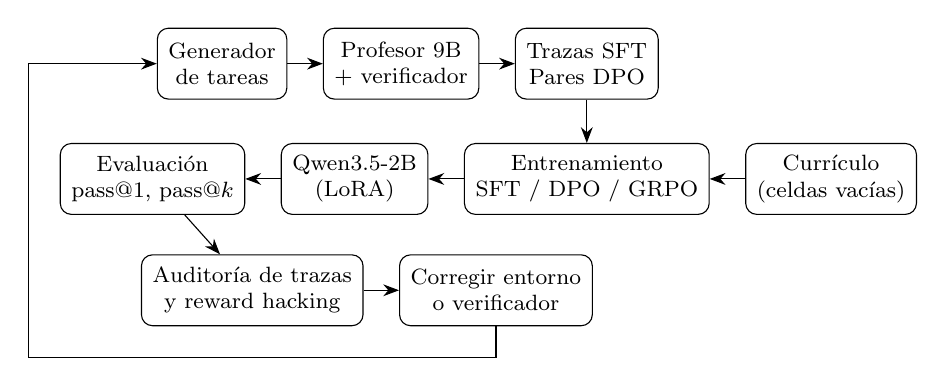
\begin{tikzpicture}[node distance=0.55cm and 0.45cm,
  b/.style={draw,rounded corners,align=center,minimum height=0.9cm,inner sep=4pt,font=\footnotesize},
  >={Stealth[length=2mm]}]
  \node[b] (gen) {Generador\\de tareas};
  \node[b,right=of gen] (prof) {Profesor 9B\\+ verificador};
  \node[b,right=of prof] (data) {Trazas SFT\\Pares DPO};
  \node[b,below=of data] (train) {Entrenamiento\\SFT / DPO / GRPO};
  \node[b,left=of train] (model) {Qwen3.5-2B\\(LoRA)};
  \node[b,left=of model] (eval) {Evaluación\\pass@1, pass@$k$};
  \node[b,right=of train] (cur) {Currículo\\(celdas vacías)};
  \node[b,below=0.5cm of model,xshift=-1.3cm] (aud) {Auditoría de trazas\\y reward hacking};
  \node[b,right=of aud] (fix) {Corregir entorno\\o verificador};
  \draw[->] (gen)--(prof); \draw[->] (prof)--(data); \draw[->] (data)--(train);
  \draw[->] (cur)--(train); \draw[->] (train)--(model); \draw[->] (model)--(eval); \draw[->] (eval)--(aud);
  \draw[->] (aud)--(fix); \draw[->] (fix.south) -- ++(0,-0.4) -| ([xshift=-4mm]eval.west) |- (gen.west);
\end{tikzpicture}
\caption{Diagrama de bloques tentativo. El verificador también es la recompensa del RL, y el currículo decide qué tareas ve el entrenamiento.}
\label{fig:bloques}
\end{figure}

\section{Cómputo y riesgos}\label{sec:computo}

Los experimentos se ejecutarán en un clúster equipado con una GPU NVIDIA RTX A6000 (48\,GB). Mientras que SFT y DPO con LoRA presentan un bajo costo computacional, GRPO es significativamente más exigente debido al muestreo en línea, por lo que acotaremos tanto la longitud máxima de las respuestas como la complejidad del entorno.

\textbf{Comparación a cómputo equivalente.} Los métodos evaluados tienen estructuras de costo distintas: SFT y DPO operan sobre conjuntos de datos estáticos, mientras que GRPO genera $G$ respuestas por \emph{prompt} antes de cada actualización. Para garantizar una comparación justa, establecemos los siguientes criterios:
\begin{itemize}
  \item \textbf{Presupuesto común ($B$):} Se define en términos de tokens procesados por el modelo objetivo (tanto generados como de entrenamiento) y horas de GPU en la A6000, acotado por la capacidad de ejecución de GRPO. El esquema secuencial SFT$\to$RLVR distribuye este mismo presupuesto $B$ entre sus dos etapas.
  \item \textbf{Curvas frente a cómputo acumulado:} Se evalúan \emph{checkpoints} en intervalos fijos de $B$ para graficar \passuno\ en función de los tokens y las horas de GPU. De este modo, la equivalencia computacional se observa directamente en la curva de aprendizaje sin depender de un único criterio de parada.
  \item \textbf{Configuración homogénea:} Todos los enfoques comparten el mismo rango de LoRA, la misma longitud máxima de respuesta y un presupuesto de evaluación idéntico.
  \item \textbf{Contabilidad separada del costo de datos:} La generación de trazas para SFT y de pares para DPO requiere inferencia del modelo profesor (9B), un gasto ausente en RLVR puro. Este costo se reportará por separado y no se descontará de $B$.
\end{itemize}

\textbf{Calibración del presupuesto $B$.} Fijamos $B = 15\text{M}$ de tokens generados por ejecución de GRPO (equivalente a unos $200$ pasos con $16$ entradas y $G=8$), con un límite máximo de $5$ horas de GPU en la A6000 por ejecución. Con la longitud de respuesta estimada, este margen permite realizar aproximadamente $16$ ejecuciones completas de GRPO. Dado que SFT y DPO consumen solo una fracción de $B$, reportaremos su gasto real sin aplicar compensaciones artificiales. Por su parte, SFT$\to$RLVR descontará el costo de la etapa supervisada de su presupuesto total $B$, y el costo de inferencia del profesor (\texttt{Qwen3.5-9B}) se mantendrá aislado del análisis comparativo. Estas estimaciones se recalibrarán en la Entrega~2 utilizando el \emph{throughput} medido en la A6000 y la longitud media de respuesta del nuevo \emph{baseline}.

\textbf{Análisis de riesgos.} A continuación, detallamos los principales riesgos técnicos y experimentales junto con sus mecanismos de detección y mitigación:
\begin{description}[leftmargin=0pt]
  \item[Ausencia de señal en RL.] GRPO actualiza la política comparando las recompensas relativas de las $G$ respuestas generadas para un mismo \emph{prompt}. Si el modelo falla o acierta sistemáticamente en todas las muestras de un grupo, las recompensas son idénticas, la ventaja se anula y el gradiente desaparece. \emph{Detección:} Monitoreo de la proporción de grupos con recompensa constante y estancamiento en la curva de recompensa inicial. \emph{Mitigación:} Restringir el entrenamiento a instancias dentro de la zona con señal, filtrar grupos sin varianza y aplicar un precalentamiento mediante SFT antes de RLVR (esquema SFT$\to$RLVR) si el modelo base carece de aciertos iniciales.

  \item[Incumplimiento del formato de salida.] Dado que el factor $\text{format}$ multiplica toda la función de recompensa, un modelo que omita o duplique el bloque \texttt{<answer>} recibirá siempre cero, anulando la señal de aprendizaje incluso cuando el razonamiento sea válido. Este problema se agrava si la generación se trunca por alcanzar el límite de tokens antes de cerrar la etiqueta. \emph{Detección:} Seguimiento de las tasas de formato válido y de truncamiento en cada experimento. \emph{Mitigación:} Aumentar la longitud máxima de generación, incluir ejemplos de formato en el \emph{prompt} (\emph{few-shot}) o inicializar el entrenamiento desde un modelo ajustado con SFT.

  \item[\emph{Reward hacking}.] La política podría descubrir atajos que incrementen la recompensa sin resolver realmente el Sudoku; por ejemplo, bajo recompensa parcial, copiar las pistas y completar el resto al azar otorga un puntaje positivo, o bien podría explotar vulnerabilidades del \emph{parser}. \emph{Detección:} Inspección periódica de trazas con alta recompensa, análisis de divergencias entre la recompensa media y la tasa real de resolución ($\text{solved}$) y auditorías manuales. \emph{Mitigación:} Diseño de pruebas unitarias adversariales (como múltiples bloques \texttt{<answer>}, texto posterior al cierre, tableros vacíos o rellenos aleatorios) que deban puntuar cero o mínimo; ante cualquier falla detectada, se parchará el verificador, se incorporará el caso a la batería de pruebas y se reentrenarán los modelos afectados.

  \item[Estancamiento o ineficacia del currículo.] Un umbral de avance $\tau$ demasiado exigente bloqueará el currículo adaptativo en las tareas más simples, mientras que uno muy laxo desplazará el entrenamiento hacia instancias sin señal. Asimismo, un resultado nulo (donde el currículo no supere al muestreo uniforme) es científicamente válido, pero debe distinguirse de una mala calibración. \emph{Detección:} Registro continuo de la distribución de dificultades muestreadas por paso. \emph{Mitigación:} Calibrar $\tau$ apoyándose en los resultados de la línea base y utilizar un calendario fijo (incremento de dificultad predeterminado por etapas) como alternativa determinista.

  \item[Escasez de instancias de entrenamiento.] El conjunto actual dispone de $50$ tareas por combinación de tamaño y nivel ($450$ en total). Bajo el presupuesto $B$, el modelo recorrerá estas instancias múltiples veces, lo que conlleva el riesgo de sobreajuste por memorización de tableros específicos en lugar de generalización. \emph{Detección:} Brecha creciente en \passuno\ entre los conjuntos de entrenamiento y prueba. \emph{Mitigación:} Generar instancias adicionales y, de ser necesario, sintetizar nuevas trazas con el modelo profesor.

  \item[Indisponibilidad o incompatibilidad de entornos externos.] Los \emph{harnesses} desarrollados por otros grupos aún no están publicados y podrían presentar barreras técnicas o un costo de evaluación prohibitivo. \emph{Mitigación:} Preseleccionar al menos dos entornos candidatos, validar su interfaz y el \passuno\ del modelo base antes de integrarlos, utilizar tareas de \emph{Reasoning Gym} como alternativa de respaldo y relegar esta evaluación a un plano secundario si surgen restricciones de tiempo.

  \item[Insuficiencia de cómputo.] Si el presupuesto de GPU resulta insuficiente para cubrir toda la matriz experimental, se perderán repeticiones con distintas semillas aleatorias, reduciendo el poder estadístico para distinguir mejoras reales del ruido. \emph{Mitigación:} Priorizar múltiples semillas en los enfoques centrales (SFT$\to$RLVR, RLVR puro y las variantes de currículo), recortar estudios de ablación secundarios antes que semillas y guardar \emph{checkpoints} frecuentes para reanudar ejecuciones interrumpidas.
\end{description}

\section{Cronograma}
\begin{center}\small
\begin{tabularx}{\linewidth}{@{}lY@{}}
\toprule
Fecha & Hito \\
\midrule
11 nov & Entrega 1: esta propuesta. \\
11--25 nov & Línea base final (cluster), datos SFT/DPO, entrenamiento de SFT y DPO, primeras curvas de recompensa GRPO. \\
25 nov & Entrega 2: informe de avance (línea base, implementación inicial, curvas de recompensa). Elegir los harness externos. \\
25 nov -- 9 dic & Caminos 3 y 4 completos, currículo y ablations, auditoría manual, redacción del paper y del póster. \\
9 dic & Entrega 3: paper (7 páginas), póster y video. \\
\bottomrule
\end{tabularx}
\end{center}

\bibliographystyle{plainnat}
\bibliography{Bibliografia}
\end{document}
